\section{Experiments results}\label{sec:expr}

The experimental study compared the presented \tool algorithm with respect to the state of the art cb100.

The benchmark consists two parts: the first one are formulae from industrial verification and the second one are random formulae. The industrial formulae are selected from SAT competition between 2002 and 2015. There are 769 industrial formulae out of 1318 formulae in these benchmarks. 388 formulae are selected from industrial formulae that a model can returned from MINISAT in 1800 seconds. The random formulae are generated from unsatisfiable random formulae using the tool of LBX \cite{MPA2015} with over 6000 formulae. For every random formulae, both \tool and cb100 are able to terminate within 1800 seconds.

In Table \ref{tab:ind}, we present the results of industrial formulae. Figure \ref{fig:ind-time} presents a plot by increasing running time of industrial instances for \tool and cb100. We categories the random benchmark into 5 groups, according to the community structure of the formula. Table 3 shows the total SAT solving time, average SAT solving time and average SAT solver call for all 3 groups. In each group, we randomly sample 20 instances and presents a plot by increasing run times in Figure \ref{fig:mcs-time}.

All algorithms introduced in this paper have been implemented in \tool, written in C++ interfacing Minisat 2.2 \cite{MINISAT}.

The experiments were conducted on a cluster of IBM iDataPlex 2.83 GHz, each instance was running with a timeout of 1800 seconds and memory limit of 8 GB.


\subsection{Industrial Experimental Results}

\begin{table*}
\centering
\begin{tabular}{ccccc}
\toprule
 &SAT Solving time&\#SAT Solving Count&Average SAT Solving Time\\
\midrule
\tool&26663 seconds &272089&0.9890 seconds\\
cb100&30295 seconds&239112&1.0174 seconds\\
\bottomrule
\end{tabular}
\caption{Experimental Results for 138 Industrial Formulae}
\label{tab:ind}
\end{table*}

SAT competitions evaluate the performance of SAT solvers, they focused on industrial formula, also contain random formulae or crafted large formulae. We select 769 industrial formulae from all benchmarks, and select 388 formulae that MINISAT return a model in 1800 seconds. The formulae are from different applications of practical, including planning, coloring, hardware/software verification, model checking and cryptanalysis.

Table \ref{tab:ind} shows the overview of industrial benchmark results. Among all the 388 instances, there are 138 instances that both \tool and cb100 were able to compute backbone within 1800 seconds.

Figure 1 provide the performance of \tool and cb100 for industrial formulae, including the time that SAT solver need to generate the first model and total SAT solving time. The first observation is that for instances that need a longer time to generate the first model, \tool outperforms cb100 in both total SAT solving time and average SAT solving time. This implies that \tool is more feasible for large formulae and reduce the complexity of SAT solving for hard formulae. For example, \tool is twice faster than cb100 when computing a formula form \emph{manthey} class. Only for formula in \emph{srhd}, \tool needed 28 more seconds than cb100 does to compute backbone, with a first SAT solving time of 437 seconds.

Another conclusion is that for formulae with first SAT solving time less than 30 seconds, \tool and cb100 are compatible, with only a few seconds more than cb100 does. cb100 highly rely on the quality of model returned by SAT solver, it performances better when SAT solver gave it a suitable model. For most of the formulae that need less than 1 second to compute a first model, both \tool and cb100 were able to compute backbone very quickly with barely difference.

In general \tool performances better than cb100 on industrial instances, especially for instances with a longer time to generate the first model, \tool have a notable advantage. Compared with cb100, we save over 20\% running time on all industrial formulae. Figure \ref{fig:ind-time} depicts the total SAT solving time of \tool and cb100 by increasing running time of cb100 for the 138 formulae. The line represents the time that a formula need to generate the first model, the running time of \tool are lines with crosses and the running time of cb100 are lines with boxes. It's easy to see that for all formulae that need 120 more seconds to generate the first model, \tool outperforms cb100.

\begin{figure}
    \centering
    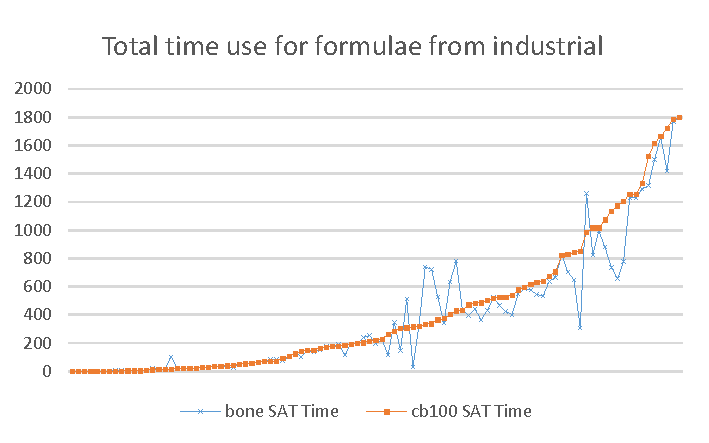
\includegraphics[scale=0.7]{ind2.pdf}
   \caption{Total time use for formulae from industrial}
   \label{fig:ind-time}
\end{figure}

\subsection{MSS Extraction Experimental Results}
In this section, the effectiveness of \tool and cb100 for MSS instances are presented.
Unlike other study that focus on the verification instances from industrial, we also study the performance of \tool and cb100 on random instances.
We propose a novel method to generate large number of random formulae, with the help of Maximal Satisfiable Subset(MSS).

Given an unsatisfiable formula $\Phi$, a subset of clauses $\Phi'\subset\Phi$ is called a MSS iff for every clause $\phi\notin\Phi'$, $\Phi'$ is satisfiable and $\Phi'\wedge\phi$ is unsatisfiable. MSS is maximal satisfiable sub-formula extracted from an unsatisfiable formula. There exist a large number of different MSS for a given unsatisfiable formula. We use LBX tool to generate MSSes from random unsatisfiable benchmark. The MSS generated are also random and with a fixed upper bound of clauses count and variables count to a given unsatisfiable formula.

Table \ref{tab:mcs} presents the overview result of MSS formulae. Inspired by the result of industrial formulae, we category MSS formulae into 5 groups according to the computing time of first model. We randomly choose 20 instances from every group and present the running time plot in Figure \ref{fig:mcs-bad}. It's strange that for random formulae, there is no clear relation between the performance of backbone computing and the computing time of first model. It's because that random formulae have more complex community structures \cite{NZG2014,LJG2015SAT,LJG015}. We use SATGraph \cite{NZW2015} tool to generate the graph of formulae in MSS benchmark. We observe that cb100 performs better on formula with a long distance single vertex in a graph, shown in \ref{fig:cb100}. On the other hand, \tool performs better on formula with a group of vertexes around the center cluster with almost the same distance from the vertexes to the center cluster. Figure \ref{fig:bone} shows an example graph of such formulae.

Based on the observation, we divide MSS benchmark into three groups according to the community structure of formulae. For formulae with a single vertex far away from center cluster, we put it to \emph{simple} group. For formulae with vertexes around the center cluster, we put it to \emph{hard} group. The rest are in \emph{medium} group. Table \ref{tab:mcs-graph} showed the result of MSS benchmark, simple(resp. medium, resp. hard) stands for the formulae in simple(resp.medium, resp. hard) group. As we can observe that \tool need less running time than cb100 does in total. However, cb100 outperforms \tool in simple group. It's because that the essence of cb100 is try to find a backbone literal by complementing models as soon as possible. The single vertex in simple formula is easy for cb100 to search. Therefore, cb100 is able to compute a backbone literal at the very early stage. With the early backbone literal, the computing is accelerated. It has been proved that the community structure of a formula related to the performance of CDCL solver \cite{NZG2014}. Our observation shown that the community structure of random formulae is also highly related to the performance of backbone computing.

\begin{figure}
    \centering
    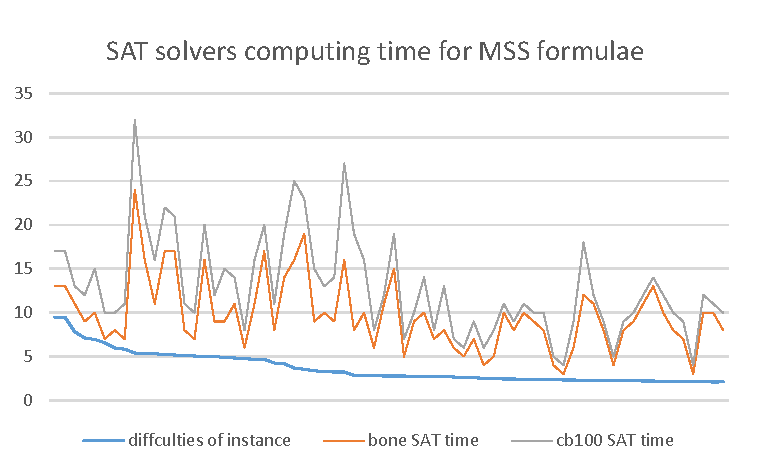
\includegraphics[scale=0.7]{mcs.pdf}
   \caption{Total time use for formulae from MCS computing}
   \label{fig:mcs-time}
\end{figure}

\begin{figure}
    \centering
    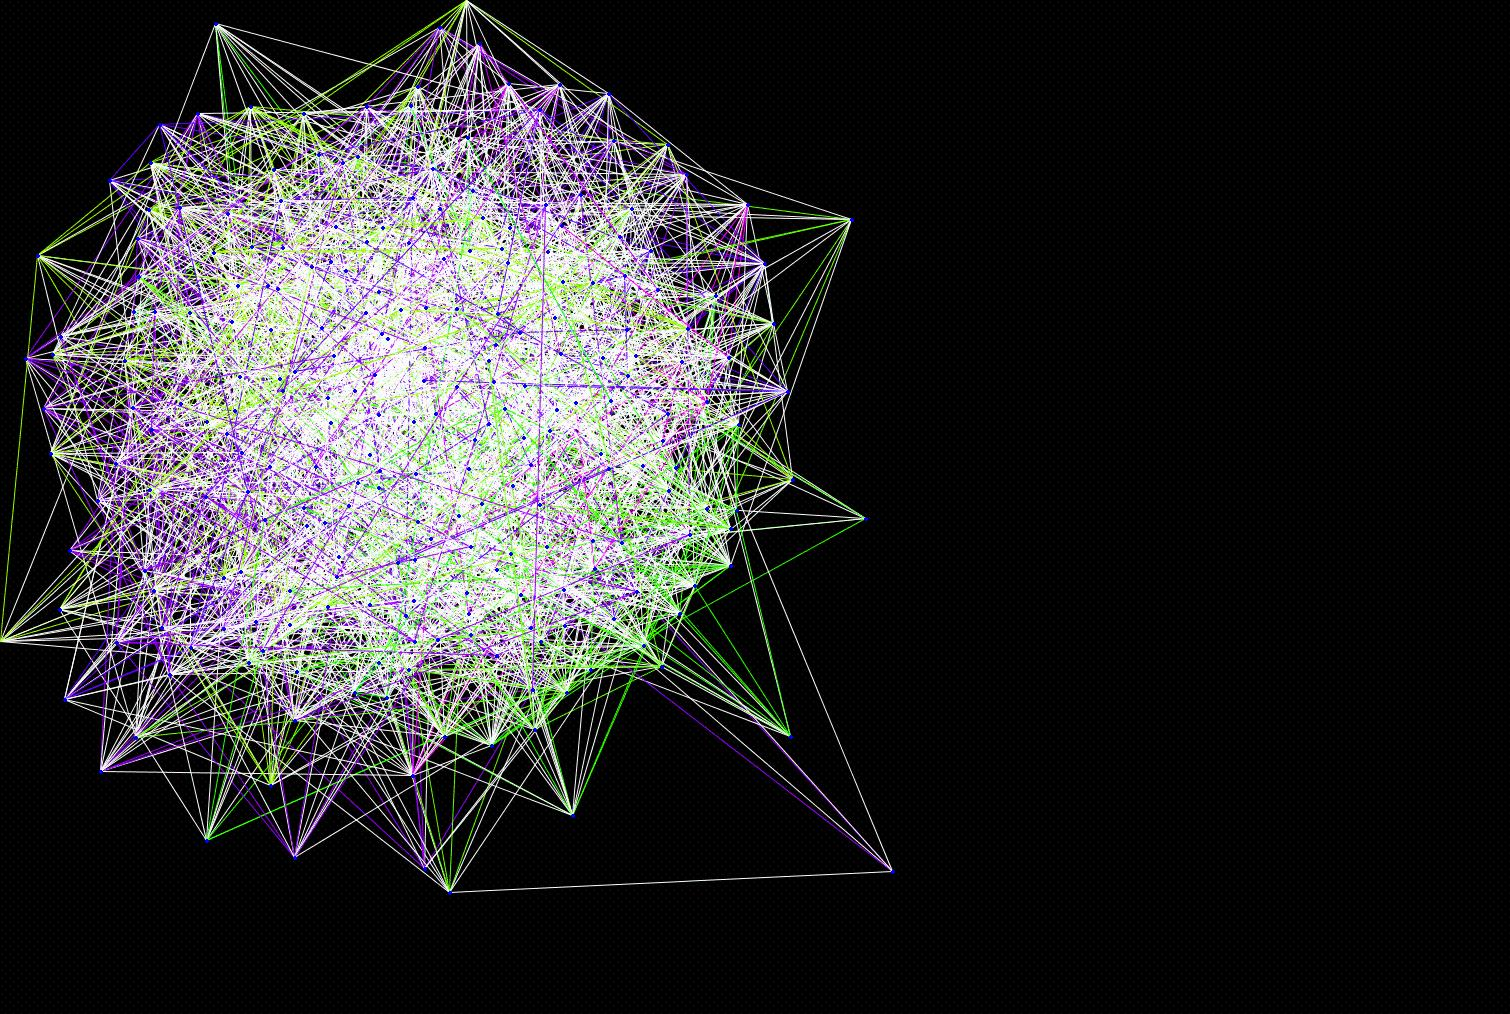
\includegraphics[scale=0.12]{cb100.jpg}
   \caption{Community Structure of Formula Performs better with cb100}
   \label{fig:cb100}
\end{figure}

\begin{figure}
    \centering
    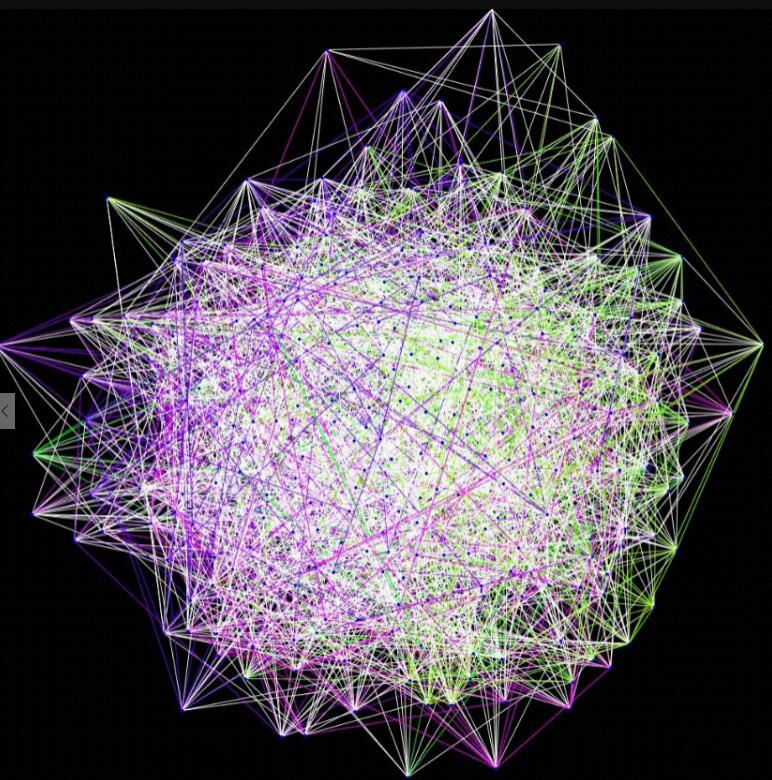
\includegraphics[scale=0.12]{bone.jpg}
   \caption{Community Structure of Formula Performs better with \tool}
   \label{fig:bone}
\end{figure}

\begin{table*}[tb]\label{tab:mcs-graph}
\caption{Results of Random Formulae}
\begin{center}
\begin{tabular}{c|c|c|c|c|c|c|c|c}
\hline \hline
\multirow{2}{*}{} & \multicolumn{2}{c|}{Total}& \multicolumn{2}{c|}{Simple} & \multicolumn{2}{c|}{Medium} & \multicolumn{2}{c}{Hard} \\
\cline{2-9}
 &SAT Time & \#SAT Count & SAT Time & \#SAT Count & SAT Time & \#SAT Count & SAT Time & \#SAT Count \\
\hline
\tool & 50183.02 sec & 1508723 & 6874.5 sec & 85570 & 35853 sec & 1332334 & 3577.9 sec & 76449 \\ \hline
cb100 & 50414.04 sec & 1532372 & 4413.5 sec & 86232 & 39040 sec & 1353258 & 5893.4 sec & 78114 \\
\hline \hline
\end{tabular}
\end{center}
\end{table*}



The results reveal that \tool is more efficient than cb100 on industrial formulae which need more than 120 seconds to compute the first model. We ran a benchmark of 6606 instances on random formulae and concludes that \tool needs less total SAT solving time than cb100 does. \tool performs better on the hard group formulae while cb100 performs better on simple group.





